\documentclass[a4paper]{amsart}

\usepackage[colorlinks=true, citecolor=red]{hyperref}  %needs to come before amsrefs package to work with \cite{}*{}
\usepackage{amssymb,latexsym}
\usepackage[alphabetic]{amsrefs}
\usepackage[mathscr]{eucal}
\usepackage{pdfsync}
\usepackage{graphicx}
\usepackage{epstopdf}
\DeclareGraphicsRule{.tif}{png}{.png}{`convert #1 `dirname #1`/`basename #1 .tif`.png}
\usepackage[all]{xy}
\usepackage{titletoc}

\CompileMatrices

\theoremstyle{plain}
\newtheorem{theorem}{Theorem}[section]
\newtheorem{lemma}[theorem]{Lemma}
\newtheorem{proposition}[theorem]{Proposition}
\newtheorem{corollary}[theorem]{Corollary}

\theoremstyle{definition}
\newtheorem{definition}[theorem]{Definition}%[section]

\theoremstyle{remark}
\newtheorem{defn}[theorem]{Definition} 
\newtheorem{example}[theorem]{Example}
\newtheorem{remark}[theorem]{Remark}
\newtheorem{discussion}[theorem]{Discussion}

\DeclareMathOperator{\Lip}{Lip}
\DeclareMathOperator{\dist}{dist}
\DeclareMathOperator{\expected}{\mathbb{E}}
\DeclareMathOperator{\prb}{Prob}
\DeclareMathOperator{\spt}{spt}
\DeclareMathOperator{\lap}{\Delta}
\DeclareMathOperator{\Tr}{Tr}

\raggedbottom

\addtolength{\textwidth}{2cm}
\addtolength{\oddsidemargin}{-1cm}
\addtolength{\evensidemargin}{-1cm} 
\addtolength{\topmargin}{-1cm} 
\addtolength{\textheight}{2cm}
% \renewcommand{\l@subsection}{\@contentsline{2}{5em}{7em}}

%\makeatletter
%\makeatother

 
%%% BEGIN DOCUMENT
\begin{document}

\title{Analysis on random fractals}  
\author{Uta Freiburg, John E.\ Hutchinson}
\date{\today}

\maketitle


%\renewcommand*\l@subsection{\@tocline{4}{50em}{7em}{10em}{10em}}


\tableofcontents

 \section{\textbf{Introduction}}

 Almost all quantities defined here will depend on the choice of a  fixed  family of IFSs $  \{ F^\lambda : \lambda \in \Lambda \}  $ and a  fixed  labelled tree $ T $, see Section~\ref{secnot}.  This dependence will not normally be made explicit.

Later we will keep $  \{ F^\lambda : \lambda \in \Lambda \}  $  fixed  but consider  different  labelled trees $ T = T(\omega) $ where $ \omega \in \Omega $.   Quantities that depend on the choice of $ T $ will be shown as functions of $ \omega $.  Frequently, but not always, there will be a probability structure $ (\Omega, \mathcal{F}, P) $ on $ \Omega $.  

\medskip Most of this consists of extending parts of \cite{Bar}*{Section 5--7, pp 60--105} to the random setting.   See also~\cite{Ham}. 

 

%%%%%%%%%%%%%%%%%%%%%%%%%%%%%%%%%%%%%%
%%%%%%%%%%%%%%%%%%%%%%%%%%%%%%%%%%%%%%%%
%%%%%%%%%%%%%%%%%%%%%%%%%%%%%%%%%%%%%%%%%%
\section{\textbf{Notation}}\label{secnot}

\subsection{Trees} A \emph{tree} $ T $  is a finitely branching rooted tree, all of whose branches have infinite length.

The branching number at the node $ w \in T $ is denoted by $ U(w) $ and the edges out of $ w $ are denoted by $ 1,2,\dots, U(w) $.  See Figure~\ref{SG23v}.

In this way each $ w \in T $ at level $ |w| =n $ can be considered  as a word $ w = w_1\dots w_n \in \mathbb{N} ^n$. 
The root node is at level $ 0 $ and corresponds to the empty word $ \emptyset $. Moreover, $ 1 \leq w_1 \leq U(\emptyset  )$,  and $ 1 \leq w_{i+1} \leq U(  w_1\dots w_i )$ for $ 1 \leq i \leq n-1 $. 

Let the set of words in $ T $ of length $ n $ be
$ T_n = \{ w \in T : |w|=n \}$.

 

\medskip
A \emph{labelled tree}   is a tree $ T $ together with a  label function  $ V:T \to   \Lambda $, where $ \Lambda $ indexes some family of IFSs:  
\begin{equation} \label{} 
 \{ F^\lambda : \lambda \in \Lambda \} , \quad  F^\lambda  = (\psi^\lambda_1, \dots, \psi^\lambda_{M_\lambda }). 
\end{equation} 
   If $ V(w) = \lambda $ then the  branching number $ U(w) $  must  equal  $ M_\lambda $.
 
The corresponding labelled tree is denoted by $ (V(w) ; w \in T ) $, or simply by $ T $.

\medskip There is usually one or more underlying probability spaces $ (\Omega, \mathcal{F}, P) $ associated with the space of labelled trees.   A tree-valued random tree is  denoted by $ T $ or $ T(\omega) $. 
If we need to distinguish between different labelled trees, even in the deterministic case where there may be no underlying probability distribution, we again use the notation $ T(\omega) $.


%%%%%%%%%%%%%%%%%%%%%%%%%%%%%%%%%%%%%%%%%
\subsection{Coding maps, points and sets}
For $ w \in T_n $  define
\begin{equation} \label{}
 \psi_w   = \psi_{w_1}^{V(\emptyset)} \circ \psi_{w_2}^{V(w_1)}\circ \dots   \circ \psi_{w_n}^{V(w_1\dots w_{n-1})} .
\end{equation} 
For $ \lambda\in \Lambda $ and $ w = w_1\dots w_n $ with $ w_i \in \{1,\dots, M_\lambda \} $ define
\[  \psi_w^\lambda    = \psi_{w_1}^\lambda \circ \psi_{w_2}^{\lambda }\circ \dots   \circ \psi_{w_n}^{\lambda } .\]

Each infinite branch of $ T $ corresponds to an \emph{infinite} word $ w $.  We write $ w \in T_\infty $  in this case.  In particular $  T_\infty  \subset \mathbb{N} ^ \mathbb{N}  $. 

The truncation of a word $ w $ (finite or infinite) to its initial segment of length $ n $ is denoted by~$ w | n = w_1\dots w_n $.

If $ w \in T_\infty $ and $ x_0 \in \mathbb{R}^n $ then under a uniform contractivity condition on the  $ F^ \lambda $ there exists $ x_w \in \mathbb{R}^n $  independent of $ x_0 $ such that 
\begin{equation} \label{} 
\psi_{w|n}(x_0) \to x_w:= \pi(w) \text{ as } n \to \infty. 
\end{equation} 
Then
\begin{equation} \label{} 
\pi(iw) = \psi_i (\pi(w)), \quad        \pi(vw) = \psi_v (\pi(w))                   .
\end{equation} 

For $ E\subset \mathbb{R}^n $    define 
\begin{equation} \label{dfe}
E_w = \psi_w (E). 
\end{equation} 

The (compact) \emph{fractal set generated by $ T $} is
\begin{equation} \label{dfk} 
K = \{ x_w : w \in T^\infty \} = \pi (T^\infty) = \lim_{n \to \infty} \bigcup_{w \in T_n} E_w 
\end{equation} 
for any compact set $ E $, where the limit is in the Hausdorff metric sense.




%%%%%%%%%%%%%%%%%%%%%%%%%%%%%%%%%%%%%%%%%%%
\section{\textbf{Uniformly pcf fractals}}\label{secupf}

For notational simplicity we consider a family of contractive IFSs 
$ \{  F^\lambda  = (\psi^\lambda_1, \dots, \psi^\lambda_{M_\lambda} ) ; \lambda \in \Lambda \} $ acting on some compact subset of $ \mathbb{R}^d $.  However, since there is no geometry involved, it is not necessary to work in Euclidean space  when working with pcf fractals as in this section, or with electric networks as in Section~\ref{secrt}.%
\footnote{In fact it is not even necessary to work in  a metric space at all, one can work in a suitable abstract symbolic framework.  See~\cite{Kig}.}
And in some ways  it is even  misleading to do so.


\subsection{Definitions}\label{secdfpcf}
\begin{figure}[htbp] %  figure placement: here, top, bottom, or page
   \centering
   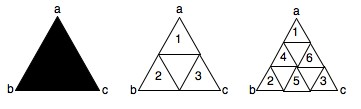
\includegraphics[width=3.5in]{SG23.jpg} 
   \caption{The set $ E $ and prefractals for $ SG(2) $ and $ SG(3) $.}
   \label{SG23}
\end{figure}


For each $ \lambda \in \Lambda $ let $ K^\lambda $ be the unique compact attractor of $ F^\lambda $. 
We say $ \{ F^\lambda : \lambda \in \Lambda \}  $ is \emph{uniformly pcf} if%
\footnote{Strictly speaking, the definition refers to the set of IFSs.   One could also say that the fractal generated by every labelled tree with labels from $ \{F^ \lambda : \lambda \in \Lambda\} $ is a pcf fractal.} 
\begin{enumerate}
 
\item For some closed set $ E $ \emph{independent} of $ \lambda $ (for example, the closure of an open set satisfying a \emph{uniform} open set condition for the $  F^\lambda $ as in Figure~\ref{SG23}), 
\begin{equation} \label{}       
\lambda \in \Lambda \Longrightarrow  \bigcup \{E^ \lambda _w :   |w|=n,\ 1\leq w_i\leq M_\lambda      \}  \downarrow K^ \lambda \text{ as } n \to \infty.
\end{equation} 
That is, the left side is a decreasing sequence of closed sets converging to the attractor $ K^ \lambda $ of $ F^\lambda  $.   

\item Let 
\begin{equation} \label{} 
B^ \lambda  = \bigcup_{i,j, i\neq j} K_i^ \lambda \cap K_j ^ \lambda  , \quad 
\Gamma^ \lambda  = \pi^{-1} (B^ \lambda ), \quad 
P   = \bigcup_{n=1}^\infty \sigma^n (\Gamma^ \lambda ),
\end{equation} 
using the notation of \eqref{dfk} and \eqref{dfe}, and where $ \sigma $ is the left shift operator.  
Then  $\Gamma^ \lambda $ (or $ B^ \lambda $) is called the \emph{criticial set} or \emph{ramification set} of the $F^ \lambda   $. 

 \emph{The set $  P  $ (or its projection $ \pi (P)\in \mathbb{R}^n   $) is required to be finite and \underline{independent} of $ \lambda $} and is called the \emph{postcritical set} or \emph{boundary set}.
 \end{enumerate} 
 
 \emph{Note} that condition (2) above may require a renumbering of the maps in the $ F^\lambda  $.  For example, with   the 6 maps in the IFS for $ SG(3) $, the maps should be listed so that the first three maps correspond to the three fixed points in $ V^{(0)} $, see~\eqref{dv0}.


Note that the definition does not require that the IFSs act on $  \mathbb{R}^n $, although that will be the case for us (at least initially). 

%%%%%%%%%%%%%%%%%%%%%%%%%%%%%%%%
\subsection{Example}  Let $ E $ be as in Figure~\ref{SG23}.  Let $ F^2 = (\psi^2_1,\psi^2_2,\psi^2_3) $ be the usual IFS for $ SG(2) $ with subscripts corresponding to Figure~\ref{SG23}.  Similarly for $ F^3 = (\psi^3_1,\dots,\psi^3_6) $ and $ SG(3) $.

Then 
\begin{align*}
 \Gamma^2&= \{ 2\dot{1}= 1\dot{2},  \   2\dot{3}= 3\dot{2}, \   3\dot{1}= 1\dot{3}\},\\
\Gamma^3&= \{ 4\dot{1}= 1\dot{2},  \   4\dot{2}= 2\dot{1}, \   2\dot{3}= 5\dot{2},
\  5\dot{3}= 3\dot{2},  \   3\dot{1}= 6\dot{3}, \   6\dot{1}= 1\dot{3},\  4\dot{3}= 5\dot{1} = 6\dot{2}  \},\\
P^2 &= P^3 =P  = \{\dot{1},\ \dot{2},\ \dot{3} \}.
\end{align*}


%%%%%%%%%%%%%%%%%%%%%%%%%%%%%%%%%%%%%%
%%%%%%%%%%%%%%%%%%%%%%%%%%%%%%%%%%%%
%%%%%%%%%%%%%%%%%%%%%%%%%%%%%%%%%%%%%%%%%%
\section{\textbf{Cells and Complexes}}  See \cite{Bar}*{p67}.

\subsection{Definitions}  

\begin{figure}[htbp] %  figure placement: here, top, bottom, or page
   \centering
   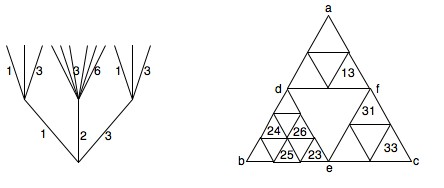
\includegraphics[width=4in]{SG23vert.jpg} 
   \caption{Using the  numbering system in Figure~\ref{SG23}, the tree $ T $ corresponds to the prefractal.
  The vertices are  $  V^{(0)} =\{a,b,c\}$, $    V^{(1)} =\{a,\dots,f\}$, $    V^{(2)} $ is the set of all vertices shown. 
Their  addresses are  respectively  $ P=\{\dot{1},\dot{2},\dot{3}\}$, 
$  P^{(1)} = \{\dot{1},    \dot{2}, \dot{3} , 1\dot{2} \& 2\dot{1}, 2\dot{3} \& 3\dot{2}, 3\dot{1} \& 1\dot{3}\}$, 
$ P^{(2)} = \{\dot{1}, 12\dot{1}\&2\dot{1}, 13\dot{1}\&11\dot{3},  \dots, 
\dot{3} \}$.
}
   \label{SG23v}
\end{figure}


Let
\begin{equation} \label{dv0} 
\begin{aligned} 
P^{(0)} &= P, & P^{(n)} &= \{ w \in T : \sigma ^n w \in P \} \text{ for } n \geq 1,\\
V^{(0)} &= \pi(P), & V^{(n)} &= \pi (P^{(n)}).
\end{aligned} 
\end{equation} 

Any set of the form $ \psi_w K = K_w $, where $ w \in T $ and $ |w|=n $, is called an \emph{$ n $-complex}.

Any set of the form $ \psi_w V^{(0)} = V_w^{(0)} $, where $ w \in T $ and $ |w|=n $, is called an \emph{$ n $-cell}.

\medskip For the following in the deterministic case see \cite{Bar}*{p68}.  Proofs are similar.


%%%%%%%%%%%%%%%%%%%%%%%%%%%%%%%%%%%%%%%%%%%%%%%
\subsection{Properties}
\begin{proposition} \label{prpupf}
Suppose $ \{ F^ \lambda : \lambda \in \Lambda \}  $ is uniformly pcf and $ T $ is a labelled tree with labels in~$ \Lambda $.

 \begin{enumerate}

\item
If $ x \in V^{(n)} $ then $ x =   \psi_w(y) $ for one or more pairs $ y \in V^{(0)} $ and $ w \in T_n  $.

\item $ V^{(n)} = \bigcup_{w\in T_n} V_w^{(0)} $.

\item If $ w\neq v \in T_n $ then $ K_w \cap K_v = V_w^{(0)} \cap  V_v^{(0)}$.

\item $ \pi^{-1}\circ \pi (P^{(n)}) = \pi^{-1} V^{(n)} = P^{(n)} $.
\item $ V^{(0)} \subset V^{(1)} \subset V^{(2)} \subset \cdots $.
\end{enumerate} 
\end{proposition} 





%%%%%%%%%%%%%%%%%%%%%%%%%%%%%%%%%%%%%%
%%%%%%%%%%%%%%%%%%%%%%%%%%%%%%%%%%%%
%%%%%%%%%%%%%%%%%%%%%%%%%%%%%%%%%%%%%%%%%%
\section{\textbf{Uniformly Nested and Affine Nested Fractals}}

%%%%%%%%%%%%%%%%%%%%%%%%%%%
\subsection{Definitions}
The family of IFSs $ \{F^ \lambda  : \lambda \in \Lambda\} $ is \emph{uniformly affine nested} if
\begin{enumerate}

\item The   family is uniformly  pcf
and   \emph{all $ F^\lambda $ act on $ \mathbb{R}^n $}.

\item The $ F^\lambda $ are affine nested fractals as in \cite{Bar}*{p69}%
\footnote{The $ \psi^\lambda  _m $ are similitudes; they satisfy the open set condition; any two 1-cells are connected by a sequence of 1-cells (\emph{connectivity}); reflection in the hyperplane bisecting the line segment joining any 2 points in the 0-cell maps $ n $-cells to $ n$=cells (\emph{symmetry});
if $ v\neq w \in T_n $ then $ K_v \cap K_w = V_v^{(0)} \cap V_w^{(0)}$ (\emph{nesting}).} 
with the additional constraint that the open set corresponding to the open set condition is independent of $ \lambda $ 

\item  \emph{The set   of essential fixed points%
\footnote{An essential fixed point is a fixed  point $ x $ such that for some $ m \neq n $ and for some fixed point $ y $,   $ \psi_m^ \lambda (x) =  \psi_n^ \lambda (y) $.} 
for each $ \lambda \in \Lambda $ is \underline{independent} of $ \lambda $} and equals $ V^{(0)}  $.%
\footnote{This is shown to be a consequence in \cite{Bar}*{p 70, Prop 5.24}.}
 \end{enumerate}
 The corresponding fractals $ K_w $ for each $ w \in T $ are said to be \emph{affine nested}.

\bigskip  The family of IFSs $ \{F^ \lambda  : \lambda \in \Lambda\} $ is \emph{uniformly nested} if
it is uniformly affine nested and if for each $ \lambda $ the maps $ \psi^\lambda _m $ all have the same contraction factor $ \alpha^ \lambda  $.
 
 

%%%%%%%%%%%%%%%%%%%%%%%%%%%%
\subsection{Properties} Suppose $ \{ F^ \lambda : \lambda \in \lambda \}  $ is uniformly affine nested.  Then
\begin{enumerate}
\item $ V^{(0)} $ is the set of essential fixed points.
\item
For each $ \lambda $,  and independently of $  \lambda $, 
\[
    P =  \{ \dot{m} : \text{ the fixed point of $  \psi^ \lambda _m $  is essential} \} .
    \] 
    
    \item Each essential fixed point is in exactly one $ n $-complex for each $ n \geq 1 $.
    
    \item Each $ 1 $-complex contains at most one essential fixed point.
\end{enumerate} 



%%%%%%%%%%%%%%%%%%%%%%%%%%%%%%%%%%%%%%
%%%%%%%%%%%%%%%%%%%%%%%%%%%%%%%%%%%%
%%%%%%%%%%%%%%%%%%%%%%%%%%%%%%%%%%%%%%%%%%
\section{\textbf{Measures on Uniformly pcf Fractals}}
Suppose $\{ F^\lambda = (\psi_1^ \lambda, \dots , \psi_{M_\lambda}^ \lambda ) : \lambda \in \Lambda \} $ is uniformly pcf.  Consider a fixed labelled tree $ T = (V,T)$.

\subsection{Definitions}
Suppose $ \theta^ \lambda = ( \theta_1^ \lambda, \dots,  \theta_{M_\lambda }^ \lambda) $ satisfies
\begin{equation} \label{} 
\sum_{m=1}^{M_\lambda} \theta^  \lambda_m= 1, \quad 1 < \theta^  \lambda_m < 1,\ \lambda \in \Lambda .
\end{equation} 
Let
\begin{equation} \label{} 
\theta_w = \theta_{w_1}^{V(\emptyset)} \theta_{w_2}^{V(w_1 )}  
  \cdot \ldots \cdot \theta_{w_n}^{V(w_1\dots w_{n-1} )}\quad  \text{for } |w|=n.
\end{equation} 



\begin{example} In Figure~\ref{SG23v} one has possible weights $ (\theta_1^2,\theta_2^2, \theta_3^2) $ and 
 $ (\theta_1^3,\dots, \theta_6^3) $. Associated to the three lowest edges in $ T $ are the weights 
 $ \theta_1^2,\theta_2^2, \theta_3^2 $.  Associated to the 12 edges at the next level are weights
 $   \theta_1^2,\theta_2^2, \theta_3^2,  \theta_1^3,\dots, \theta_6^3,  \theta_1^2,\theta_2^2, \theta_3^2$\, respectively.  Associated to each $ w \in T_n $ is the weight obtained by multiplying the weights of the $ n $ edges in $ w $.
 \end{example} 
 
\begin{example}  Suppose $\{ F^\lambda : \lambda \in \Lambda \} $ is uniformly affine nested with the similitudes $\psi_m^ \lambda $  having contraction ratios $ \alpha _m ^ \lambda $. Then the natural weights are 
  \[
  \theta_m^ \lambda = ( \alpha _m ^ \lambda )^ \beta,   \quad \text{where } 
                \sum_{m=1}^{M_\lambda}  ( \alpha _m ^ \lambda )^ \beta = 1.
                \]
 For the uniformly nested case where each $ \psi^ \lambda _m $ has contraction ratio $ \alpha ^ \lambda $  independent of $ m $, it is natural to take $ \theta_m^ \lambda = (M_ \lambda )^{-1} $.
 
  \bigskip
 \emph{Define}  $\widetilde{\mu} =  \widetilde{\mu}_\theta $ as the natural product measure on $ T_\infty $,  given on cylinder sets by
 \[   \widetilde{\mu}_\theta \{ v \in T_\infty : v|n = w \} = \theta_{w}. \]
 
 \emph{Define} $ \mu = \mu_\theta $ on the fractal $ K $ corresponding to $ T $  by
 \[ \mu = \mu_\theta = \pi_{\#} \widetilde{\mu}. \]
 It is defined on the collection of Borel sets $ \mathcal{B}(K) $, which is generated by the cylinder sets $  K_w $ for $ w \in T  $, i.e.
 \[   \mu_\theta (K_w) = \theta_w . \]
 \end{example} 
 
%%%%%%%%%%%%%%%%%%%%%%%%%%%%%%%%%%%% 
\subsection{Properties} 
Essentially from the definitions
 \begin{equation} \label{} 
  \int_Kf\, d\mu  = \sum_{w\in T_n} \theta_w \int f \circ \psi_w\, d \mu, \quad 
 \mu  = \sum_{w\in T_n} \theta_w \psi_{w\#} \mu,
\end{equation}
 where $  \psi_{w\#} \mu $ is the pushforward  measure given by
 $   \psi_{w\#} \mu (E) = \mu( \psi_w^{-1} E) $.
 
 \bigskip  We define $ \mu_n $ to be the measure on $ V^{(n)} $ obtained by pushing the $ \mu $-mass on each $ n $-complex $ K_w $ onto its boundary $ V_w^{(0)} $.  

Let $ N_0 = \# V^{(0)} $, the number of vertices in $ V^{(0)} $. For $ x \in V^{(n)} $  \emph{define}
\begin{equation} \label{}
  \mu_n(x) = \frac{1}{N_0} \sum_{w\in T_n} \theta_w  \mathcal{X}_{V_w^{(0)}}(x) .
\end{equation} 
That is, $ x \in V^{(n)} $ obtains a contribution $ \theta _w/N_0 $ from each $ n $-complex $ V_w^{(0)} $ to which it belongs.

Then
\begin{equation} \label{} 
\mu_n \rightharpoonup \mu,
\end{equation} 
since for continuous $ f $ on $ K $,
\begin{align*}
\left| \int f\, d\mu - \int f\, d\mu_n \right|   &\leq  
     \sum_{w \in T_n}  \left| \int_{K_w} f\, d\mu - \int_{K_w} f\, d\mu_n \right|  \\
     &  \leq  \sum_{w \in T_n}   \mu_n(K_w) \max_{x,y \in K_w } |f(x) - f(y)|  \\
      &\leq \max\{|f(x) - f(y)| :  w \in T_n,\ x,y \in K_w \} \to 0,
\end{align*} 
using uniform continuity for the last inequality.

%%%%%%%%%%%%%%%%%%%%%%%%%%%%%%%%%%%%%%
%%%%%%%%%%%%%%%%%%%%%%%%%%%%%%%%%%%%
%%%%%%%%%%%%%%%%%%%%%%%%%%%%%%%%%%%%%%%%%%
\section{\textbf{Replication and Trace for a Single IFS}}\label{secrt}

\subsection{Assumptions}
Consider a \emph{single} pcf IFS  $F = (\psi_1,\dots, \psi_M) $, see Section~\ref{secupf}.

\medskip Assume the following intersection condition:
\begin{equation} \label{intcon}
\parbox{5in}{ \emph{Any two distinct $ 1 $-cells $ \psi  _m (V^{(0)}) $ and $ \psi  _n (V^{(0)}) $ intersect in at most one point.} }
\end{equation}
The set of intersection points    is   the critical set $ B^ \lambda $ from Proposition~\ref{prpupf}(3), and from (2) in Section~\ref{secdfpcf}.   See Figure~\ref{SG23v}.

The assumption holds in the cases of interest here, although it is not known if it holds in general for nested fractals, see \cite{Bar}*{p71 (5.16)}.  
 
  \medskip  Let $ \rho  = ( \rho _1,\dots, \rho _{M })$  where $ \rho  _m > 0 $.  Then $ \rho  $ is called a \emph{resistance scaling vector}.  
  
\begin{example}  \label{exinv}  For the IFS corresponding to $ SG(2) $ the natural value is $ \rho = (\frac{5}{3}, \frac{5}{3}  , \frac{5}{3} ) $ and for $ SG(3) $ it is $   \rho = (\frac{15}{7}, \dots  , \frac{15}{7} ) $.   See Section *** .
\end{example} 

%%%%%%%%%%%%%%%%%%%%%%%%%%%%%%
\subsection{Definition of Replication}  \label{secdfr} Suppose  for $ 1 \leq m \leq M $ that $ V^{(0)} \subset W^m $ where $ W^m $ is finite  and $ (W^m,A^m) $ is a network with conductance matrix $ A^m = (a^m_{xy}) $. Let $ \mathcal{E}_m $ be the  Dirichlet form on $ (W^m,A^m) $.


 In particular, the case $ W^m= V^{(0)} $ for all $ m $ is important.  
 
\medskip
 \emph{Assume} for $ m \neq n $ that 
\begin{equation} \label{wint}
 \psi  _m (W^m) \cap \psi  _n (W_n) =  \psi  _m (V^{(0)}) \cap \psi  _n (V^{(0)}) .
\end{equation} 
Thus copies of   $ W^m $ are   joined together by joining   the corresponding copies  of $ V^{(0)} $ in the standard manner  to form $ V^{(1)} $, but no other nodes are joined.
This is true, for example,  if $ W^m\subset E$, where $ E $ is the set used in the Definition from  Section~\ref{secdfpcf} after replacing $ F^ \lambda $ by $ F $.
  
\medskip   Informally, the  \emph{replication network  $(W^R , A^ R ) $       using $ (F,\rho ) $} is obtained by
multiplying the conductances   $ a^m_{xy} $ by $ \rho_m   $, applying    $ \psi   _m $ to   $ W^m $, and joining the resulting networks together at their common vertices (which form the critical subset of $ V^{(1)}$).
Note that 
\begin{equation} \label{} 
V^{(0)} \subset W^m\ \forall m , \quad V^{(0)} \subset V^{(1)}\subset W^R.
\end{equation} 
The \emph{corresponding Dirichlet form} on $ (W^R,A^R) $ is denoted by~$ \mathcal{E} ^R = \mathcal{E} _A^R$.

 \medskip More precisely:
\begin{defn}  The  \emph{replication network  $(W^R , A^ R ) $       using $ (F,\rho ) $} is given  by
\begin{equation} \label{dfrn}
\begin{aligned}
W^R  &  = \bigcup_{m=1}^{M } \psi  _ m (W^m),\\
 a_{xy} ^R  &= 
 \begin{cases}
       \rho _m a^m_{vw} & 
       \text{if }  x\neq y,\ v,w\in V^{(0)}, \  \psi  _ m(v) = x,\   \psi _ m(w) = y \\
            0                                    & \text{otherwise},
            \end{cases} \\
  a_{xx}^R  &= \sum\{\rho   _m a^m_{vv} :  \psi  _ m(v) = x  \}.
  \end{aligned}
  \end{equation} 
  \end{defn} 
Concerning the definition of $ a_{xy}^R $, note that by assumption there is at most one  $ m $ and one pair $ {v,w} $ satisfying the condition used in the  definition of $ a_{xy}^R  $.   Concerning $ a^R_{xx} $, there will be more than one  $ m $ and $ v $ precisely when $ x $ is in the critical set.
  
  
  %%%%%%%%%%%%%%%%%%%%%%%%%%%%%%%%%% 
\subsection{Invariance under Replication} 
 \begin{defn} Suppose $ (V^{(0)}, A)$  is a network on $  V^{(0)} $ with replication network $ (V^{(0)}, A^R)$ under $ (F,\rho) $ as in Section~\ref{secdfr}.  Then   $ (V^{(0)}, A)$ is \emph{invariant under replication} if%
\footnote{For trace networks see \cite{Hut}.}  
\[
A = \Tr (A^R \mid V^{(0)} ).
\] 
\end{defn}  

Example~\ref{exinv} gives an example of an invariant network if $ B = \begin{bmatrix} -2 & 1 & 1 \\ 1 & -2 & 1 \\ 1 & 1  & -2 \end{bmatrix} $.




%%%%%%%%%%%%%%%%%%%%%%%%%%%%%%%%%% 
\subsection{Properties of Replication}  

Suppose a network is obtained by replication as in the previous section, with resistance scalings $ \rho_m $. The following Proposition shows the following:
\begin{enumerate}
\item  The  Dirichlet energy of a function $ f $ defined on the replicated   network can be  obtained from the  Dirichlet energy of the    corresponding function  on each of the original networks by  scaling   these energies with $ \rho_m $  and summing.


\item The trace of the replicated network on $ V^{(1)} $ is the same as the replication of the traces   on $ V^{(0)}$ of the original networks.
\end{enumerate} 


\begin{proposition} \label{proptr} Suppose $ F =(\psi_1,\dots, \psi_m) $ is a pcf fractal satisfying the intersection condition~\eqref{intcon}, and $ \rho = (\rho_1,\dots,\rho_M) $ is a resistance scaling vector.

Suppose   $ (W^m,A^m) $ is a network with conductance matrix $ A^m = (a^m_{xy}) $ for $ 1 \leq m \leq M $.
Suppose   $ V^{(0)} \subset W^m $ for all $ m $ and  $ \psi  _m (W^m) \cap \psi  _n (W_n) =  \psi  _m (V^{(0)}) \cap \psi  _n (V^{(0)}) $ for $ m\neq n $.
 
Let the replication network $ (W^R, A^R ) $ be defined  by~\eqref{dfrn}. 
 
Then the matrix $ A^R $ is a conductance matrix.  
The  Dirichlet form $ \mathcal{E}_A ^R $ is given by 
\begin{equation} \label{repm}
\mathcal{E} _A^R  (f,g)= \frac{1}{2} \sum_{x,y} a_{xy}^R\big(f(x) - f(y) \big) \big( g(x) - g(y) \big) 
= \sum_{m=1}^{M  } \rho_m \mathcal{E}_m (f \circ \psi_m , g \circ \psi_m  ) .
\end{equation} 


Suppose  $ B^m = \Tr(A^m\mid V^{(0)}) $. 
Let $ (V^{(1)},B^R) $ be the replication network obtained by applying $ \psi_m $ and $ \rho_m $ to $ (V^{(0)},B^m) $ for $ 1 \leq m \leq M $. Then $ B^R = \Tr(A^R\mid V^{(1)}) $.
\end{proposition} 

\begin{proof}  It is clear $ a^R_{xy} \geq 0 $ for $ x \neq y $.  Moreover,
\begin{align*}
\sum_{\{y:y \neq x\}} a^R_{xy}&
  = \sum_{\{m\, :\, x \in V_m^{(0)}\}} \sum_{ \{y \, : \,  y \in V_m^{(0)},\,  y \neq x \} } a^R_{xy}
  \intertext{(each $ y \neq x $ is counted once on the right side by \eqref{wint} and the initial assumption about he intersection of $ 1 $-cells)}
  &=  \sum_{\{m\, :\, x \in V_m^{(0)}\}}  \sum_{ \{w \, : \,  w \in V ^{(0)},\,  w \neq \psi_m^{-1}(x)  \} } 
                            \rho_m a _{\psi_m^{-1}(x)\, w}\\
  &=- \sum_{\{m\, :\, x \in V_m^{(0)}\}}  \rho_m  a _{\psi_m^{-1}(x)\, \psi_m^{-1}(x)}  \\
  &= -a^R_{xx}.
  \end{align*} 
Hence $ A^R $ is a conductance matrix.

\medskip The first equality in \eqref{repm} is by definition. The second is by splitting the first sum  into disjoint sums  over the sets $ V_m^{(0)}$.

\medskip For the final claim it is sufficient to show that if $ g : V^{(1)} \to \mathbb{R} $ and $ f $ is its harmonic extension to $ (W^R,A^R) $ then
\[
\mathcal{E}_B^R(g) = \mathcal{E} _A^R(f). 
\]

But $ f $ is the harmonic extension of $ g $ to $ (W^R,A^R) $  iff,  for every $ m $,  $ f\circ \psi_m $ is the harmonic extension  of $ g\circ \psi_m : V^{(0)} \to \mathbb{R} $ to $ (W^m,A^m) $.
To see this, consider $ x \in W\setminus V^{(1)} $ and let $ m $ be the unique integer such that $ x \in \psi_m(W^m) $, see \eqref{wint}.  Then $ g $ is harmonic at $ x $ iff $ g \circ \psi_m $  is harmonic at $ \psi_m^{-1}(x) $, because all relevant conductances are scaled by the same factor $ \rho_m $.
\end{proof} 

\begin{corollary}
  Continue the assumptions of Proposition~\ref{proptr}.
Suppose $ (V^{(0)} , B) $ is invariant under replication and $ \Tr(A^m\mid V^{(0)}) = B $ for all $ m $. 

Then $ \Tr (A^R\mid V^{(0)} ) = B $.
\end{corollary} 

\begin{proof}
\begin{align*}
\Tr(A^R \mid V^{(1)}) &= B^R \quad \text{by Proposition~\ref{proptr},} \\
\Tr(B^R \mid V^{(0)}) &= B  \quad \text{by assumption,} \\
\therefore\ \Tr(A^R \mid V^{(0)}) &= B \quad \text{by the tower property of traces.} \qedhere \\
\end{align*}
 \end{proof} 
 
 
 
 
 
 
 
%%%%%%%%%%%%%%%%%%%%%%%%%%%%%%%%%%%%%%
%%%%%%%%%%%%%%%%%%%%%%%%%%%%%%%%%%%%
%%%%%%%%%%%%%%%%%%%%%%%%%%%%%%%%%%%%%%%%%%
\begin{thebibliography}{9} 



\bib{Bar}{article}{
   author={Barlow, Martin T.},
   title={Diffusions on fractals},
   conference={
      title={Lectures on probability theory and statistics},
      address={Saint-Flour},
      date={1995},
   },
   book={
      series={Lecture Notes in Math.},
      volume={1690},
      publisher={Springer},
      place={Berlin},
   },
   date={1998},
   pages={1--121},
%   review={\MR{1668115 (2000a:60148)}},
}

\bib{Ham}{article}{
   author={Hambly, B. M.},
   title={Brownian motion on a random recursive Sierpinski gasket},
   journal={Ann. Probab.},
   volume={25},
   date={1997},
%   number={3},
   pages={1059--1102},
 %  issn={0091-1798},
 %  review={\MR{1457612 (98i:60072)}},
}

\bib{Hut}{article}{
   author={Hutchinson, J. E.},
   title={Electric Currents, Random Walks and Analysis on Graphs},
   note={Informal Notes}
   date={2009}
}   
   
   

\bib{Kig}{book}{
   author={Kigami, Jun},
   title={Analysis on fractals},
   series={Cambridge Tracts in Mathematics},
   volume={143},
   publisher={Cambridge University Press},
%   place={Cambridge},
   date={2001},
   pages={viii+226},
%   isbn={0-521-79321-1},
%   review={\MR{1840042 (2002c:28015)}},
}



\end{thebibliography}

\end{document}

